%=========================================================================
% (c) Michal Bidlo, Bohuslav Křena, 2008

\chapter{Úvod}
Abychom mohli napsat odborný text jasně a~srozumitelně, musíme splnit několik základních předpokladů:
\begin{itemize}
\item Musíme mít co říci,
\item musíme vědět, komu to chceme říci,
\item musíme si dokonale promyslet obsah,
\item musíme psát strukturovaně. 
\end{itemize}

Tyto a další pokyny jsou dostupné též na školních internetových stránkách \cite{fitWeb}.

Přehled základů typografie a tvorby dokumentů s využitím systému \LaTeX je 
uveden v~\cite{Rybicka}.

\section{Musíme mít co říci}
Dalším důležitým předpokladem dobrého psaní je {\it psát pro někoho}. Píšeme-li si poznámky sami pro sebe, píšeme je jinak než výzkumnou zprávu, článek, diplomovou práci, knihu nebo dopis. Podle předpokládaného čtenáře se rozhodneme pro způsob psaní, rozsah informace a~míru detailů.

\section{Musíme vědět, komu to chceme říci}
Dalším důležitým předpokladem dobrého psaní je psát pro někoho. Píšeme-li si poznámky sami pro sebe, píšeme je jinak než výzkumnou zprávu, článek, diplomovou práci, knihu nebo dopis. Podle předpokládaného čtenáře se rozhodneme pro způsob psaní, rozsah informace a~míru detailů.

\section{Musíme si dokonale promyslet obsah}
Musíme si dokonale promyslet a~sestavit obsah sdělení a~vytvořit pořadí, v~jakém chceme čtenáři své myšlenky prezentovat. 
Jakmile víme, co chceme říci a~komu, musíme si rozvrhnout látku. Ideální je takové rozvržení, které tvoří logicky přesný a~psychologicky stravitelný celek, ve kterém je pro všechno místo a~jehož jednotlivé části do sebe přesně zapadají. Jsou jasné všechny souvislosti a~je zřejmé, co kam patří.

Abychom tohoto cíle dosáhli, musíme pečlivě organizovat látku. Rozhodneme, co budou hlavní kapitoly, co podkapitoly a~jaké jsou mezi nimi vztahy. Diagramem takové organizace je graf, který je velmi podobný stromu, ale ne řetězci. Při organizaci látky je stejně důležitá otázka, co do osnovy zahrnout, jako otázka, co z~ní vypustit. Příliš mnoho podrobností může čtenáře právě tak odradit jako žádné detaily.

Výsledkem této etapy je osnova textu, kterou tvoří sled hlavních myšlenek a~mezi ně zařazené detaily.

\section{Musíme psát strukturovaně} 
Musíme začít psát strukturovaně a~současně pracujeme na co nejsrozumitelnější formě, včetně dobrého slohu a~dokonalého značení. 
Máme-li tedy myšlenku, představu o~budoucím čtenáři, cíl a~osnovu textu, můžeme začít psát. Při psaní prvního konceptu se snažíme zaznamenat všechny své myšlenky a~názory vztahující se k~jednotlivým kapitolám a~podkapitolám. Každou myšlenku musíme vysvětlit, popsat a~prokázat. Hlavní myšlenku má vždy vyjadřovat hlavní věta a~nikoliv věta vedlejší.

I k~procesu psaní textu přistupujeme strukturovaně. Současně s~tím, jak si ujasňujeme strukturu písemné práce, vytváříme kostru textu, kterou postupně doplňujeme. Využíváme ty prostředky DTP programu, které podporují strukturovanou stavbu textu (předdefinované typy pro nadpisy a~bloky textu). 


\chapter{Proteíny}

Proteíny (bielkoviny) môžeme charakterizovať ako základné stavebné prvky všetkých živých organizmov. Nie sú však iba stavebnými prvkami bunky, zabezpečujú väčšinu bunečných funkcií. Pochopenie procesu vzniku proteínov a ich funkcie nachádza široké uplatnenie v odvetviach ako medicína, poľnohospodárstvo, priemysel a mnohé ďaľšie. 
V tejto kapitole sa budem zaoberať základným rozdelením proteínov, procesom ich vzniku z DNA a štruktúrou.

\section{Základné rozdelenie proteínov}

Proteíny sú biopolyméry tvorené z jedného alebo viacerých polypeptidových reťazcov, ktoré je možné chápať ako sekvenciu polymérov aminokyselín navzájom spojených kovalentnou peptidovou väzbou. Proteíny sa skladajú do množstva komplikovaných tvarov a~ich funkcie súvisia s~konkrétnym priestorovým usporiadaním (konformáciou), pričom sa snažia zaujať čo najlepšiu konformáciu z energetického hľadiska. Konformácia vychádza z~primárnej štruktúry, ktorú môžeme chápať ako reťazec aminokyselín v~danom poradí \cite{proteiny}. Podľa funkcie môžeme proteíny rozdeliť do niekoľkých skupín \cite{proteiny}:  
\begin{itemize}
	\item \textbf{Enzýmy:} ich funkciou je katalýza rozpadu a tvorba kovalentných väzieb. Príkladom môže byť napríklad pepsín, ktorý sa podieľa na odbúraní bielkovín pri trávení.
	\item \textbf{Štruktúrne proteíny:} tvoria základné stavebné jednotky buniek a tkanív, poskytujú im mechanickú oporu. Príkladom je keratín tvoriaci základnú zložku vlasov a nechtov.
	\item \textbf{Transportné proteíny:} prenášajú malé molekuly a ionty v organizme. Príkladom sú proteín hemoglobín ako nosič kyslíka v krvnom obehu a proteín transferrin prenášajúci železo.
	\item \textbf{Pohybové proteíny:} sú pôvodcami pohybu buniek a tkanív. Príkladom takýchto proteínov sú kinesin a myosin.
	\item \textbf{Zásobné proteíny:} slúžia na skladovanie malých molekúl a iontov. Kasein v mlieku poskytuje zdroj aminokyselín pre novonarodené živočíchy. 
	\item \textbf{Signálne proteíny:} ich funkcoiu je prenos informačných signálov medzi bunkami. Do tejto skupiny patrí známy proteín inzulín regulujúci hladinu cukru v krvi.
	\item a ďaľšie.
\end{itemize}

\section{Aminokyseliny}
Aminokyseliny sú odvodené od organických kyselín a predstavujú rôzne triedy molekúl s~jednou spoločnou vlastnosťou, všetky vlastnia karboxylovú (COOH) a aminovú ($NH_{2}$) skupinu. Tieto skupiny sú naviazané k jednému uhlíkovému atómu, ktorý je označovaný ako $\alpha$ uhlík. Rôznorodosť jednotlivých aminokyselín spočíva v~postrannom reťazci (R) určujúcom chemické vlastnosti aminokyselín, resp. proteínov. Jednotlivé aminokyseliny sú v~proteínovej molekule vzájomne spojené peptidovou väzbou, ktorá prepojuje karboxylovú skupinu jednej aminokyseliny s~amino skupinou druhej. Reťazec viacerých aminokyselín je označovaný ako peptidový reťazec (polypeptid). 
Celkovo existuje 20 rôznych aminokyselín, ktoré môžeme na základe chemických vlastností postranných reťazcov rozdeliť na šesť základných skupín \cite{aminokyseliny}:

\begin{itemize}
	\item \textbf{Aminokyseliny s alifatickým postranným reťazcom:} alanin (Ala), valin (Val), leucin (Leu), isoleucin (Ile), glycin (Gly)
	\item \textbf{Bazické skupiny s aminovou skupinou na postrannom reťazci:} arginin (Arg), lysin (Lys)
	\item \textbf{S aromatickým jadrom alebo hydroxylovou skupinou na postrannom reťazci:}
	histidin (His), fenylalanin (Phe), serin (Ser), threonin (Thr), tyrosin (Tyr), tryptofan (Trp)
	\item \textbf{Kyslé skupiny s karboxylovou alebo aminovou skupinou na postrannom reťazci:} kyselina asparagová (Asp), asparagin (Asn), kyselina glutamová (Glu), glutamin (Gln)
	\item \textbf{So sírou v postrannom reťazci:} methionin (Met), cystein (Cys)
	\item \textbf{Obsahujúce sekundárny amin:} prolin (Pro)
\end{itemize}

\section{Syntéza proteínov}

Proteíny vznikajú z DNA v procese nazývanom proteosyntéza. Tento proces sa skladá z 2 hlavných častí, ktorými sú transkripcia a translácia.

\begin{itemize}

\item \textbf{Transkripcia:} pri procese transkripcie dochádza k prepisu časti nukleotidovaj sekvencie DNA (génu) do molekuly RNA. Dôležitú úlohu zohráva enzým RNA-polymeráza, ktorá musí pred začiatkom traskripcie nájsť oblasť tzv. promotoru obsahujúcu informáciu o začiatku transkripcie a následne sa na túto oblasť naviazať. Proces prepisu končí keď RNA-polymeráza narazí na sekvenciu tzv. terminátoru. Výsledná molekula RNA sa označuje ako mediátorová RNA (mRNA). 
\item \textbf{Translácia:} pri procese translácie dochádza k prenosu informácie z mRNA do polypeptidového reťazca aminokyselín. Sekvencia nukleotidov RNA sa postupne číta po trojiciach (tzv. kodónoch), pričom každý kodón je preložený na jednu z dvadsiatich aminokyselín. Trojica nukleotidov umožňuje vytvoriť 64 možných kombinácií, takže jedna aminokyselina môže byť reprezentovaná viacerými kodónmi. Výsledkom translácie je proteín.

\end{itemize}
\newpage
\section{Štruktúra proteínov}
Popis trojrozmernej štruktúry proteínov môžeme podľa \cite{aminokyseliny} rozdeliť do štyroch úrovní organizácie:

\begin{itemize}
	\item \textbf{Primárna štruktúra:} sekvencia aminokyselín v polypeptidovom reťazci
	\item \textbf{Sekundárna štruktúra:} zachytáva elementy, ktoré na krátkych úsekoch v~sekvencií proteínu zaujímajú podobnú konformáciu. Ide najmä o $\alpha$\--špirálu ($\alpha$\--helix) a $\beta$\--~štruktúra alebo ($\beta$\--skladaný list). $\alpha$\--špirála je také priestorové usporiadanie, kedy reťazec vytvára špirálu. Táto konformácia je stabilizovaná vodíkovými mostíkmi medzi peptidovými väzbami ležiacimi nad sebou \cite{bibid}. V prípade $\beta$\--štruktúry prebiehajú úseky reťazca paralelne vedľa seba a~sú stabilizované vodíkovými mostíkmi medzi susediacimi úsekmi.
	\item \textbf{Terciálna štruktúra:} reprezentuje trojrozmerné priestorové usporiadanie zloženého polypeptidového reťazca \cite{aminokyseliny}. Na podobe výslednej terciálnej štruktúry majú vplyv chemické vlastnosti aminokyselín a ich usporiadanie v reťazci. 
	\item \textbf{Kvartérna štruktúra:} popisuje usporiadanie jednotlivých polypeptidových reťazcov v molekule proteínu. Týka sa to však iba tzv. oligomerných proteínov, ktoré sú tvorené z viac ako jedného polypetidového reťazca.
	
	Primárnu, sekundárnu, terciálnu a kvartérnu štruktúru je možné vidieť na obrázku \ref{struktura}:
\end{itemize}
\begin{figure}[H]
		\begin{center}
		\scalebox{0.5}
		{   
			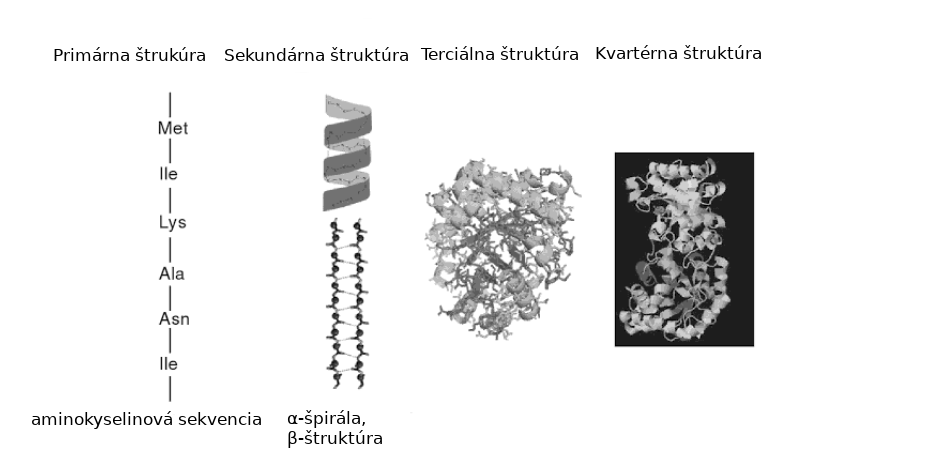
\includegraphics{structure.png}
		}
		\caption{Primárna, sekundárna, terciálna a kvartérna štruktúra. Prevzaté a upravené z \cite{gromiha}.}
		\label{struktura}
	\end{center}
\end{figure}

\chapter{Vplyv aminokyselinových substitúcií na stabilitu proteínu}

Stabilita je jednou z najdôležitejších vlastností proteínu. Motivácia skúmania stability je dnes veľká, pretože táto vlastnosť proteínov je dôležitá v mnohých oblastich ako je medicína, kde chceme dosiahnuť výrobu účinnejších liečiv, v oblasti priemyslu a poľnohospodárstva. Stabilný proteín dokáže lepšie znášať nepriaznivé podmienky okolitého prostredia, akými sú vyššie teploty alebo chemické vlastnosti okolia v ktorom sa proteín nachádza. Na stabilitu proteínu však vplývajú aminokyselinové substitúcie, ktoré môžu proteín stabilizovať, ale aj destabilizovať. Preto vzniká potreba skúmať vplyv substitúcií na stabilitu. V tejto kapitole sa zmienim o stabilite proteínu, čo stabilitu určuje a o dôvodoch vzniku a vplyve mutácií.


\section{Stabilita proteínu}
Stabilita proteínu je určená množinou vzájomne pôsobiacich a ovplyvňujúcich sa síl. Tieto sily určujú, či sa proteín nachádza vo svojom pôvodnom zloženom alebo rozloženom (denaturovanom) stave. Stabilita je úzko prepojená so stavom, v ktorom sa proteín nachádza. Stabilný proteín sa nachádza v zloženom stave, ktorý je stabilizovaný rôznymi vzájomnými interakciami, kde patria hydrofóbne, elektrostatické, vodíkové väzby alebo van der Waalsove sily. Naopak, nestabilný proteín sa nachádza v denaturovanom stave, kde dominuje entropická a neentropická voľná energia. \cite{gromiha}

Stabilitu proteínu je možné reprezentovať ako zmenu tzv. Gibbsovej (voľnej) energie ($\Delta$G) potrebnej na prechod proteínu zo zloženého do denaturovaného stavu alebo naopak. 
Gibbsova voľná energia je termodynamický potenciál vyjadrujúci maximálne množstvo reverzibilnej práce, ktorá môže byť uskutočnená termodynamickým systémom pri konštantnej teplote a tlaku. Gibbsova voľná energia je definovaná nasledujúcim vzťahom \cite{gibbs}:
\begin{align}
	G = H - TS,
\end{align}
kde $H$ predstavuje entalpiu, $T$ teplotu a $S$ entropiu.

  Existuje niekoľko laboratórnych metód na určenie stability ako napríklad cirkulárny dichroizmus (CD), diferencilna skenovacia kalorimetria (DSC), fluorescencia (Fl), absorpcia svetla (Abs), nukleárna magnetická rezonancia (NMR) \cite{gromiha}.

Určenie stability bez použitia niektorej z laboratórnych metód je možné uskutočniť výpočtom jedného z existujúcich silových polí (Talaris, Score12, ...). Výpočet takéhoto poľa ukazuje nasledujúci jednoduchý príklad \cite{free_energy} \cite{gromiha}:

Voľná energia v zloženom stave je daná vzťahom  
	\begin{align}
		G_{F} = G_{hy} + G_{el} + G_{hb} + G_{vw} + G_{ss},
	\end{align}

kde $G_{hy}, G_{el}, G_{hb}, G_{ss}, G_{vw}$ sú hydrofóbne, elektrostatické, vodíkové, disulfidické a van der Waalsove voľné energie. 

Hydrofóbnu voľnú energiu je možné odhadnúť z dostupnej rozpustnosti. Vypočítaná je podľa vzťahu
	\begin{align}
	G_{hy} =  \varSigma \Delta \sigma_{i}[A_i (folded) - A_i (unfolded)],
	\end{align}

kde $i$ predstavuje rôzne typy atómov, $A_i (folded)$ a $A_i (unfolded)$ sú dostupné povrchové plochy (ASA) jednotlivých typov atómov v zloženom a nezloženom stave a $\sigma_{i}$ reprezentuje atómové solvatačné parametre.

Elektrostatickými interakciami najviac prispievajú nabité postranné reťazce reziduí Lysine, Hystodine, Arginine a kyselina asparagová a glutamová.

Vodíkové väzby sú jednými z hlavných zúčastnených pri tvorbe sekundárnej štruktúry proteínu. Výpočet ich príspevku je založený najmä na ich geometrických informáciách.

Van der Waalsove energie je možné vypočítať zjednotením Lennard-Jonesovho potenciálu ako
	\begin{align}
	G_{vw} = (A_{ij} /r^{12}_{ij} - B_{ij} /r^{6}_{ij}),
\end{align}
kde $A_{ij} = \varepsilon^{*}_{ij}(R^{*}_{ij})^{12}$, $B = 2\varepsilon^{*} (R^{*})^{6}$, $R^{*} = (R^{*} + R^{*})$,  $\varepsilon^{*} = (\varepsilon^{*} \varepsilon^{*}).$ $R^{*}$ a $\varepsilon^{*}$ sú van der Waalsov rádius a hĺbka TODO.

Voľná energia v nezloženom stave je daná vzťahom

\begin{align}
	G_U = G_{en} + G_{ne},
\end{align}
kde $G_{en}$ a $G_{ne}$ sú entropické a neentropické voľné energie.


\section{Mutácie}
Na stabilitu proteínu vplývajú aminokyselinové mútacie, ktoré môžu spôsobiť to, že proteín sa stane nestabilným. Preto do hlavnej oblasti skúmania stability patrí predikcia zmeny stability na základe aminokyselinovej mutácie. Jedná sa o predikciu zmeny Gibbsovej voľnej energie ($\Delta\Delta$G) medzi voľnou energiou pôvodného a zmutovaného proteínu. Môžeme ju definovať nasledujúcim vzťahom:
\begin{align}
	G_U = G_{mutant} - G_{original},
\end{align}
Podľa tejto hodnoty je možné rozdeliť mutácie na stabilizujúce, neutrálne a destabilizujúce. Väčšia snaha pri predikcií môže viesť k zlepšeniu návrhu nových odolnejších proteínov alebo pri štúdií rozličných chorôb.

Mutácie sú náhodné alebo cielené zmeny v DNA. Sú naprosto nevyhnutné pre biologickú evolúciu, bez nich by sa skôr či neskôr zastavila. Ak by sa výraznejšie zmenili podmienky vonkajšieho prostredia, organizmy by bez mutácií nemuseli na zmeny zareagovať a pravdepodobne by vyhynuli. Mutáciami sú označované všetky také zmeny genetickej informácie, ktoré nie sú výsledkom segregácií a rekombinácií už existujúcich častí genotypov \cite{mutace}. 
Podľa úrovne, na ktorej sa mutácia vyskytla, môžeme rozlišovať \cite{flegr}:
\begin{itemize}
	\item \textbf{Génové mutácie:} zmena v stavbe DNA, ktorá je reprezentovaná zmenou nukleotidovej sekvencie na určitom mieste \cite{mutace}. Nazývajú sa tiež bodovými mutáciami a z hľadiska predikcie sú najzásadnejšie.
	\item \textbf{Chromozómové mutácie:} mení sa štruktúra chromozómu.
	\item \textbf{Genónové mutácie:}  mení sa počet chromozómov.
\end{itemize}

\subsection{Vznik mutácií}

Mutácie nevznikajú náhodne, každá mutácia má svoju príčinu za ktoru stojí pôsobenie tzv. mutagénnych faktorov. Medzi najdôležitejšie patria chemické a fyzikálne faktory.

Medzi fyzikálne faktory patria rôzne zdroje žiarenia, najmä ionizujúce a ultrafialové. Poškodenie štruktúry DNA je priamo úmerné množstvu absorbovaného žiarenia.

Medzi chemické faktory môžeme zaradiť genotoxické látky, tzv. genotoxíny. Takýchto látok je veľké množstvo a patria medzi ne napríklad pesticídy, herbicídy, niektoré farbivá, konzervačné a dezinfekčné látky \cite{mutace}. 

\subsection{Typy mutácií}

Podľa \cite{flegr} rozlišujeme tri základné typy génových mutácií:
\begin{itemize}
	\item \textbf{Substitúcia:} jedná sa o zámenu jedného alebo viacerých párov po sebe nasledujúcich bází inými \cite{mutace}. V tomto prípade sa nemení dĺžka pôvodného proteínu. Novovziknutý proteín sa obvykle líši v jednej aminokyseline oproti pôvodnému. 
	\item \textbf{Vloženie:} jedná sa o vloženie jedného alebo viacerých nových párov bází do pôvodnej sekvencie, spôsobuje zväčšenie dĺžky sekvencie.
	\item \textbf{Odstránenie:} odstránenie jedného alebo viacerých po sebe nasledujúcich párov bází, mení dĺžku sekvencie rovnako ako inzercia.
\end{itemize}

\begin{figure}[H]
	\centering
	\begin{center}
		\scalebox{0.6}
		{   
			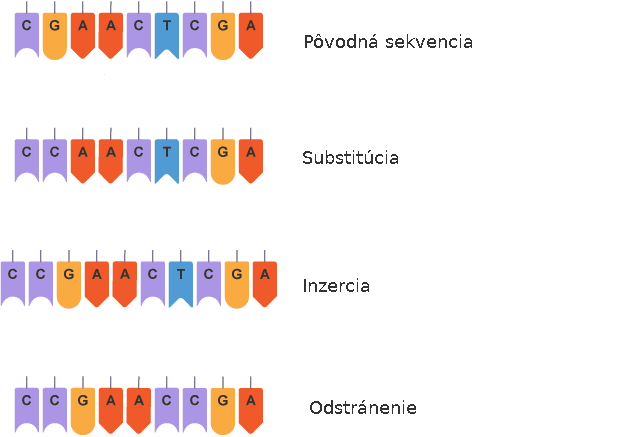
\includegraphics{mutation_types.png}
			%https://www.bbc.co.uk/education/guides/zc499j6/revision/2
		}
		\caption[mutacie]{Jednotlivé typy mutácií\footnotemark.}
	\end{center}
\end{figure}
\footnotetext{Zdroj: \url{https://www.bbc.co.uk/education/guides/zc499j6/revision/2}}

V prípade, že k mutácií dôjde v kódujúcej oblasti, môžeme mutácie rozlíšiť na \cite{flegr}:
\begin{itemize}
	\item \textbf{Synonymné:} vychádzajú z tzv. degenerovanosti genetického kódu. Zámena nukleotidu v kodóne sa tak na štruktúre proteínu nemusí vôbec prejaviť a vyzerá to tak, ako keby k mutácií vôbec nedošlo. 
	\item \textbf{Nesynonymné:} pri zmene nukleotidu v kodóne dochádza k zmene aminokyseliny a rovnako aj k zmene konformácie proteínu.
	\item \textbf{Posunové:} spôsobujú zmenu čítacieho rámca a často vedú k predčasnému ukončeniu prekladu proteínu.
	\item \textbf{Nezmyselné:} vytvárajú STOP kodón a tým spôsobujú predčasné ukončenie prekladu proteínu.
\end{itemize}

\chapter{Strojové učenie}

Strojové učenie je v súčasnej dobe chápané ako disciplína umelej inteligencie. Základnou technikou strojového učenia je prehľadávanie stavového priestoru. K charakteristickým rysom patrí využívanie znalostí, práca so symbolickými či štruktúrovanými premennými \cite{machine_learning}. Pojem strojové učenie takisto označuje počítačové metódy pracujúce s obrovským množstvom dát, medzi ktorými sa snažia nájsť vzťahy. Takéto metódy nachádzajú svoje uplatnenie pri hľadaní riešení v mnohých odvetviach akými sú počítačové videnie, rozpoznávanie reči a takisto bioinformatika. Keďže strojové učenie nachádza v mnohých odvetviach čoraz väčšie uplatnenie, je potrebné brať do úvahy jeho výhody a rovnako aj nevýhody. Medzi výhody patrí automatické hľadanie vzťahov vo veľkom množstve dát, čo by bolo pri mechanickom hľadaní takmer nemožné. Medzi hlavné nevýhody metód patrí neschopnosť správnej analýzy dát pri nevyváženosti predložených dát, nesprávne výsledky pri malom množstve testovacích dát pre metódu alebo nemožnosť práce s dátami obsahujúcimi veľké množstvo parametrov.

V tejto kapitole sa budem venovať základným technikám strojového učenia, popisom používaných algoritmov. Priestor bude venovaný aj technikám zlepšujúcim základné postupy strojového učenia a nástrojom pre predikciu stability využívajúcich strojové učenie.

\section{Úvod do strojového učenia}

Podľa \cite{alpaydin} je možné algoritmy strojového učenia rozdeliť do 3 základných skupín:
\begin{itemize}
	\item klasifikácia
	\item regresia
	\item hľadanie asociácií
\end{itemize}

Klasifikácia rieši problém priradenia výstupnej triedy vstupným dátam, ktoré môžu byť reprezentované vektorom hodnôt. Ako príklad je možné si predstaviť zatriedenie žiadateľov o pôžičku do tried s vysokým alebo nízkym rizikom toho, že pôžičku nebudú schopní splácať na základe rôznych údajov o nich.

Regresné metódy narozdiel od klasifikačných nepriraďujú vstupom výstupnú triedu, ale snažia určiť rovno číselnú hodnotu výstupu. Príkladom môže byť určenie ceny ojazdeného auta na základe parametrov ako počet najazdených kilometrov, značka, rok výroby.

Asociačné pravidlá slúžia na hľadanie zaujímavých asociácií vo veľkom objeme dát. Pri ich hľadaní nás zaujíma podmienená pravdepodobnosť, ktorá sa uvádza vo forme $P(X|Y)$, $Y$ je produkt podmienený výskytom produktu $X$.

Metódy strojového učenie môžeme ďalej rozdeliť na základe spôsobu, akým sa učia. Podľa \cite{alpaydin} ich rozdeľujeme na:
\begin{itemize}
	\item \textbf{Učenie s učiteľom:} Pri tomto type učenia je nutné mať k dispozícií vstupné aj výstupné dáta. Cieľom je nájsť vzťahy medzi vstupom a výstupom, ktoré slúžia na naučenie metódy. Medzi algoritmy patriace do tejto skupiny radíme regresiu aj klasifikáciu.
	\item \textbf{Učenie bez učiteľa:} V tomto type učenie nie sú k dispozícií referenčné výstupné dáta, ale len vstupné. Snahou je nachádzať pravidelnosti vo vstupných dátach. Medzi takéto metódy patria rôzne typy zhlukovania. 
\end{itemize}

\section {Rozhodovacie stromy}
Rozhodovací strom je hierarchický model so stromovou štruktúrou. Metódy tohto typu používajú učenie s učiteľom a môžeme ich použiť na klasifikáciu aj regresiu. Štruktúra stromu je tvorená z dvoch typov uzlov, vnútorných (nelistových) a listových uzlov. Každý z nelistových uzlov implementuje testovaciu funkciu. Po vyhodnotení tejto funkcie sa vyberie nasledujúci uzol v ktorom sa bude pokračovať. Tento proces začína v koreňovom uzle a pokračuje rekurzívne až do dosiahnutia listového uzlu. Listový uzol obsahuje označenie triedy do ktorej bude zaradený vstupný vektor alebo číselnú hodnotu.

\subsection{Algoritmus J48}

Algoritmus J48 patrí k metódam rozhodovacích stromov. Algoritmus produkuje klasifikačno-rozhodovací strom pre poskytnuté dáta rekurzívnym rozdeľovaním dát. Rozhodnutie rastie použitím stratégie depth-first. Algortimus berie do úvahy všetky možné testy, ktoré môžu rozdeliť dáta a vyberá test udávajúci najlepšiu informačnú hodnotu. Pre každý diskrétny atribút je zvážený jeden test s výsledkami pre taký počet hodnôt koľko je rôznych hodnôt atribútov. 

\subsection{Algoritmus Náhodný strom (Random Tree)}

Pri tomto algoritme je strom náhodným stromom vytvoreným náhodne z množstva potenciálne možných stromov. Každý list obsahuje $k$ náhodných parametrov. Náhodné vytvorenie stromu v tomto kontexte znamená, že každý strom v množine steomov má rovankú šancu byť vybratý. Kombinácia veľkého počtu náhodných stromov obvykle vedie k správnemu modelu. 

\subsection{Algoritmus Náhodný les (Random Forest)}

Random Forest je metóda založená na kombinácií viacerých rozhodovacích stromov. Každý strom závisí na hodnotách náhodného vektora hodnôt navzorkovaného nezávisle a s rovnakým rozložením pre všetky stromy v tzv. lese stromov. Prvýkrát bola metóda predstavená v práci \cite{breiman}. Obecne môžeme metódu popísať nasledujúcou definíciou:

Náhodný les (random forest) je klasifikátor tvorený kolekciou klasifikátorov so stromovou štruktúrou $\{h(x,\Theta_{k}), k=1, ...\}, $ kde $\{k\}$ sú nezávisle identicky rozdelené náhodné vektory a každý strom hlasuje jednotlivo o najpopulárnejšej triede vo vstupe $x$.
\newpage
Najväčší pozornosť tejto metódy tvoria 3 vlastnosti:
\begin{itemize}
	\item poskytuje presnú predikciu pre mnohé typy aplikácií
	\item je schopná merať dôležitosť jednotlivých parametrov pri trénovaní modelu
	\item blízkosť medzi vzorkami môže byť merané trénovaným modelom
\end{itemize} 

Algoritmus random forest pre klasifikáciu aj regresiu môžeme zjednodušene popísať nasledovne, pričom uvažujeme $M$ rozhodovacích stromov. Schéma metódy je znázornená na obrázku \ref{random_forest}:
\begin{itemize}
	\item Pre každý z $M$ rozhodovacích stromov vytvoríme sadu trénovacích dát z originálnych dát. Na ich výber slúži metóda tzv. bagging, ktorá náhodne vyberie zadaný počet trénovacích dát.
	\item Pre každú množinu trénovacích dát vytvoríme klasifikačný alebo regresný strom, ktorý je následne natrénovaný na $M$-tej náhodnej množine trénovacích dát. V tejto metóde je každý uzol rozdelený najlepším rozdelením spomedzi podmnožiny prediktorov vybraných náhodne v tomto uzle. Naopak pri klasických stromoch je uzol rozdelený na základe najlepšieho rozdelenia medzi všetkými premennými.
	\item Predikcia nových dát spojením výsledkov predikcie M stromov, napríklad hlasovaním väčšiny (tzv. majority voting) pri klasifikácií alebo priemerom hodnôt pri regresií.
\end{itemize}

Rozšírenie algoritmu random forest je momentálne veľmi aktívnou oblasťou vo výpočetnej biológií. Metóda nachádza veľké uplatnenie v bioinformatike, napríklad aj pri nástrojoch predikujúcich stabilitu proteínov.

\begin{figure}[H]
	\centering
	\begin{center}
		\scalebox{0.8}
		{   
			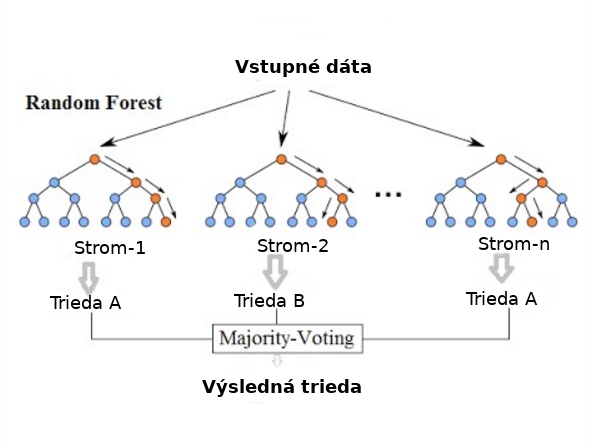
\includegraphics{rf.png}
			%https://d2wh20haedxe3f.cloudfront.net/sites/default/files/random_forest_diagram_complete.png
		}
		\caption[Random Forest]{Metóda Random Forest\footnotemark.}
		\label{random_forest}
	\end{center}
\end{figure}
\footnotetext{Zdroj: \url{http://bit.ly/2rpjSDK}}

\section {Support vector machines (SVM)}

Support vector machines patria k najnovším metódam strojového učenia. Tieto metódy uskutočňujú klasifikáciu konštruovaním N-dimenzionálnej nadroviny, ktorá optimálne rozdeľuje dáta do dvoch kategórií. Cieľom je teda nájsť takú nadrovinu, ktorá rozdelí vstupné vektory tak, že jedna skupina vektorov je na jednej strane roviny a druhá na strane opačnej. Vektory nachádzajúce sa blízko nadroviny označujeme ako tzv. podporné vektory (support vectors). 

Ak sú trénovacie dáta lineárne rozdeliteľné, potom pár $(\textbf{w},b)$ existuje ako 

	$\textbf{w}^{T}\textbf{x}_{i} + b \geq 1$, pre všetky $\textbf{x}_{i} \in P$
	
    $\textbf{w}^{T}\textbf{x}_{i} + b \leq -1$, pre všetky $\textbf{x}_{i} \in N$
    
s rozhodovacím pravidlom daným vzťahom $f_{\textbf{w},b} ( x ) = sgn(\textbf{w}^{T}x + b )$, kde $\textbf{w}$ je váhový vektor a $b$ je odchýlka (tzv. bias).

V prípade, že dáta sú lineárne separovateľné do dvoch tried, optimálnu nadrovinu je možné nájsť minimalizovaním štvorcovej normy rozdeľujúcej nadroviny. Jedná sa o konvexný kvadratický programovací problém.
Pri možnosti lineárneho rozdelenia sa SVM snaží nájsť 1-dimenzionálnu nadrovinu (priamku), ktorou rozdelí skupiny vstupných vektorov. Po rozdelení dát priamkou metóda zistí vzdialenosť priamky od najbližších podporných vektorov. Táto vzdialenosť sa označuje ako tzv. krajná hranica (margin), pričom sa hľadá najväčšia vzdialenosť medzi podpornými vektormi.  

Lineárne rozdeliteľné dáta sú však len ideálnym príkladom. Ak by analýza pozostávala len z premenných z dvoch kategórií, dvoch predikovaných premenných a množiny bodov rozdeliteľných priamkou, bolo by to veľmi jednoduché. V skutočnosti sa tieto metódy musia vysporiadať s viac ako dvomi predikovanými premennými, rozdelením dát nelineárnymi krivkami alebo množinami dát, ktoré nemôžeme úplne rozdeliť. 

\subsection{Jadrové funkcie}

Pri väčšine reálnych problémov neexistuje lineárna nadrovina rozdeľujúca pozitívne a negatívne vzorky v trénovacích dátach. Jedným z riešení je namapovanie dát do priestoru, ktorý má viac dimenzí a definovať rozdeľujúcu nadrovinu v tomto priestore. Takýto viacdimenzionálny priestor sa nazýva priestor transformovaných vlastností. S vhodne vybraným priestorom transformovaných vlastností dostatočnej dimenzie, akúkoľvek trénovaciu dátovú sadu je možné rozdeliť.
Mapovanie dát do iného (potencionálne nekonečného) Hilbertovho priestoru H je definované ako $\Phi:R^{d} \rightarrow H$. Trénovací algoritmus bude potom závisieť len na dátach skrz bodové produkty v H, napríklad na funkciách v tvare $\Phi(x_{i})\cdot\Phi(x_{j})$. Ak by existovala tzv. jadrová funkcia K taká, že $K(x_{i},x_{j}) = \Phi(x_{i})\cdot\Phi(x_{j})$, v algoritme by sme potrebovali iba K. 

Jadrové funkcie sú špeciálnou triedou funkcií umožňujúce výpočet vnútorných produktov priamo v priestore vlastností bez nutnosti mapovania dát tak ako to bolo popísané vyššie. 
Akonáhle je vytvorená nadrovina, jadrová funkcia je použitá na mapovanie nových bodov do priestoru vlastností pre klasifikáciu.
\newpage
Výber vhodnej aproximačnej jadrovej funkcie je dôležitý, pretože funkcia definuje transformovaný priestor vlastností v ktorom budú klasifikované trénovacie dáta. Medzi najpoužívanejšie jadrové funkcie patria
\begin{itemize}
	\item $K(x,y) = (x \cdot y + 1)^{P}$
	\item $K(x,y) = e^{- {\parallel x - y \parallel}^{2}/ {2\sigma}^{2}}$
	\item $K(x,y) = tanh (\kappa x \cdot y -\delta)^{P}$
\end{itemize}


\subsection{Algoritmus SMO}

Sekvenčná minimalizačná optimalizácia (SMO) je algoritmus na trénovanie SVM, ktorý jednoducho rieši kvadratický SVM problém. SMO uskutočňuje dekompozíciu celkového problému na podproblémy riešené analyticky. Metóda si v každom kroku vyberá na vyriešenie najmenší optimalizačný problém. Pre typický kvadratický SVM problém, najmenší možný optimalizačný problém zahŕňa dva Lagraengove násobitele. V každom kroku si metóda vyberia dva tieto násobitele na spoločnú optimalizáciu, nájde pre ne optimálne hodnoty a aktualizuje SVM. Výhodou tohto algoritmu je, že množstvo potrebnej pamäte pri trénovacej sade je lineárne, čo umožňuje algoritmu pracovať s veľkými trénovacími sadami. 
 
\section{Algoritmus Naive Bayes}

Naive Bayes je klasifikačným algoritmom pre klasifikačné problémy, kde sa vyskytujú dve alebo viac tried. Je založený na Bayesovom teoréme s nezávislými predpokladmi medzi prediktormi. Klasifikátor predpokladá, že efekt hodnoty $x$ prediktoru na danú triedu $c$ je nezávislý na hodnotách ďaľších prediktorov. Predpoklad sa nazýva triedna podmienená nezávislosť. 

Tento model je jednoduchý na vytvorenie, no napriek svojej jednoduchosti klasifikátor často poskytuje dobré výsledky a je široko používaný, pretože v mnohých prípadoch prekonáva komplikovanejšie klasifikačné metódy.

\section{Ensemble metódy}

\section{Nástroje pre predikciu stability využívajúce strojové učenie}

\chapter{Typografické a~jazykové zásady}
Při tisku odborného textu typu {\it technická zpráva} (anglicky {\it technical report}), ke kterému patří například i~text kvalifikačních prací, se často volí formát A4 a~často se tiskne pouze po~jedné straně papíru. V~takovém případě volte levý okraj všech stránek o~něco větší než pravý -- v~tomto místě budou papíry svázány a~technologie vazby si tento požadavek vynucuje. Při vazbě s~pevným hřbetem by se levý okraj měl dělat o~něco širší pro tlusté svazky, protože se stránky budou hůře rozevírat a~levý okraj se tak bude oku méně odhalovat.

Horní a~spodní okraj volte stejně veliký, případně potištěnou část posuňte mírně nahoru (horní okraj menší než dolní). Počítejte s~tím, že při vazbě budou okraje mírně oříznuty.

Pro sazbu na stránku formátu A4 je vhodné používat pro základní text písmo stupně (velikosti) 11 bodů. Volte šířku sazby 15 až 16 centimetrů a~výšku 22 až 23 centimetrů (včetně případných hlaviček a~patiček). Proklad mezi řádky se volí 120 procent stupně použitého základního písma, což je optimální hodnota pro rychlost čtení souvislého textu. V~případě použití systému LaTeX ponecháme implicitní nastavení. Při psaní kvalifikační práce se řiďte příslušnými závaznými požadavky.

Stupeň písma u~nadpisů různé úrovně volíme podle standardních typografických pravidel. 
Pro všechny uvedené druhy nadpisů se obvykle používá polotučné nebo tučné písmo (jednotně buď všude polotučné nebo všude tučné). Proklad se volí tak, aby se následující text běžných odstavců sázel pokud možno na {\it pevný rejstřík}, to znamená jakoby na linky s~předem definovanou a~pevnou roztečí.

Uspořádání jednotlivých částí textu musí být přehledné a~logické. Je třeba odlišit názvy kapitol a~podkapitol -- píšeme je malými písmeny kromě velkých začátečních písmen. U~jednotlivých odstavců textu odsazujeme první řádek odstavce asi o~jeden až dva čtverčíky (vždy o~stejnou, předem zvolenou hodnotu), tedy přibližně o~dvě šířky velkého písmene M základního textu. Poslední řádek předchozího odstavce a~první řádek následujícího odstavce se v~takovém případě neoddělují svislou mezerou. Proklad mezi těmito řádky je stejný jako proklad mezi řádky uvnitř odstavce.

Při vkládání obrázků volte jejich rozměry tak, aby nepřesáhly oblast, do které se tiskne text (tj. okraje textu ze všech stran). Pro velké obrázky vyčleňte samostatnou stránku. Obrázky nebo tabulky o~rozměrech větších než A4 umístěte do písemné zprávy formou skládanky všité do přílohy nebo vložené do záložek na zadní desce.

Obrázky i~tabulky musí být pořadově očíslovány. Číslování se volí buď průběžné v~rámci celého textu, nebo -- což bývá praktičtější -- průběžné v~rámci kapitoly. V~druhém případě se číslo tabulky nebo obrázku skládá z~čísla kapitoly a~čísla obrázku/tabulky v~rámci kapitoly -- čísla jsou oddělena tečkou. Čísla podkapitol nemají na číslování obrázků a~tabulek žádný vliv.

Tabulky a~obrázky používají své vlastní, nezávislé číselné řady. Z toho vyplývá, že v~odkazech uvnitř textu musíme kromě čísla udat i~informaci o~tom, zda se jedná o~obrázek či tabulku (například \uv{\ldots {\it viz tabulka 2.7} \ldots}). Dodržování této zásady je ostatně velmi přirozené.

Pro odkazy na stránky, na čísla kapitol a~podkapitol, na čísla obrázků a~tabulek a~v~dalších podobných příkladech využíváme speciálních prostředků DTP programu, které zajistí vygenerování správného čísla i~v~případě, že se text posune díky změnám samotného textu nebo díky úpravě parametrů sazby. Příkladem takového prostředku v~systému LaTeX je odkaz na číslo odpovídající umístění značky v~textu, například návěští ($\backslash${\tt ref\{navesti\}} -- podle umístění návěští se bude jednat o~číslo kapitoly, podkapitoly, obrázku, tabulky nebo podobného číslovaného prvku), na stránku, která obsahuje danou značku ($\backslash${\tt pageref\{navesti\}}), nebo na literární odkaz ($\backslash${\tt cite\{identifikator\}}).

Rovnice, na které se budeme v~textu odvolávat, opatříme pořadovými čísly při pravém okraji příslušného řádku. Tato pořadová čísla se píší v~kulatých závorkách. Číslování rovnic může být průběžné v~textu nebo v~jednotlivých kapitolách.

Jste-li na pochybách při sazbě matematického textu, snažte se dodržet způsob sazby definovaný systémem LaTeX. Obsahuje-li vaše práce velké množství matematických formulí, doporučujeme dát přednost použití systému LaTeX.

Mezeru neděláme tam, kde se spojují číslice s~písmeny v~jedno slovo nebo v~jeden znak -- například {\it 25krát}.

Členicí (interpunkční) znaménka tečka, čárka, středník, dvojtečka, otazník a~vykřičník, jakož i~uzavírací závorky a~uvozovky se přimykají k~předcházejícímu slovu bez mezery. Mezera se dělá až za nimi. To se ovšem netýká desetinné čárky (nebo desetinné tečky). Otevírací závorka a~přední uvozovky se přimykají k~následujícímu slovu a~mezera se vynechává před nimi -- (takto) a~\uv{takto}.

Pro spojovací a~rozdělovací čárku a~pomlčku nepoužíváme stejný znak. Pro pomlčku je vyhrazen jiný znak (delší). V~systému TeX (LaTeX) se spojovací čárka zapisuje jako jeden znak \uv{pomlčka} (například \uv{Brno-město}), pro sázení textu ve smyslu intervalu nebo dvojic, soupeřů a~podobně se ve zdrojovém textu používá dvojice znaků \uv{pomlčka} (například \uv{zápas Sparta -- Slavie}; \uv{cena 23--25 korun}), pro výrazné oddělení části věty, pro výrazné oddělení vložené věty, pro vyjádření nevyslovené myšlenky a~v~dalších situacích (viz Pravidla českého pravopisu) se používá nejdelší typ pomlčky, která se ve zdrojovém textu zapisuje jako trojice znaků \uv{pomlčka} (například \uv{Další pojem --- jakkoliv se může zdát nevýznamný --- bude neformálně definován v~následujícím odstavci.}). Při sazbě matematického mínus se při sazbě používá rovněž odlišný znak. V~systému TeX je ve zdrojovém textu zapsán jako normální mínus (tj. znak \uv{pomlčka}). Sazba v~matematickém prostředí, kdy se vzoreček uzavírá mezi dolary, zajistí vygenerování správného výstupu.

Lomítko se píše bez mezer. Například školní rok 2008/2009.

Pravidla pro psaní zkratek jsou uvedena v~Pravidlech českého pravopisu \cite{Pravidla}. I~z~jiných důvodů je vhodné, abyste tuto knihu měli po ruce. 


\section{Co to je normovaná stránka?}
Pojem {\it normovaná stránka} se vztahuje k~posuzování objemu práce, nikoliv k~počtu vytištěných listů. Z historického hlediska jde o~počet stránek rukopisu, který se psal psacím strojem na speciální předtištěné formuláře při dodržení průměrné délky řádku 60 znaků a~při 30 řádcích na stránku rukopisu. Vzhledem k~zápisu korekturních značek se používalo řádkování 2 (ob jeden řádek). Tyto údaje (počet znaků na řádek, počet řádků a~proklad mezi nimi) se nijak nevztahují ke konečnému vytištěnému výsledku. Používají se pouze pro posouzení rozsahu. Jednou normovanou stránkou se tedy rozumí 60*30 = 1800 znaků. Obrázky zařazené do textu se započítávají do rozsahu písemné práce odhadem jako množství textu, které by ve výsledném dokumentu potisklo stejně velkou plochu.

Orientační rozsah práce v~normostranách lze v~programu Microsoft Word zjistit pomocí funkce {\it Počet slov} v~menu {\it Nástroje}, když hodnotu {\it Znaky (včetně mezer)} vydělíte konstantou 1800. Do rozsahu práce se započítává pouze text uvedený v~jádru práce. Části jako abstrakt, klíčová slova, prohlášení, obsah, literatura nebo přílohy se do rozsahu práce nepočítají. Je proto nutné nejdříve označit jádro práce a~teprve pak si nechat spočítat počet znaků. Přibližný rozsah obrázků odhadnete ručně. Podobně lze postupovat i~při použití OpenOffice. Při použití systému LaTeX pro sazbu je situace trochu složitější. Pro hrubý odhad počtu normostran lze využít součet velikostí zdrojových souborů práce podělený konstantou cca 2000 (normálně bychom dělili konstantou 1800, jenže ve zdrojových souborech jsou i~vyznačovací příkazy, které se do rozsahu nepočítají). Pro přesnější odhad lze pak vyextrahovat holý text z~PDF (např. metodou cut-and-paste nebo {\it Save as Text\ldots}) a~jeho velikost podělit konstantou 1800. 


\chapter{Závěr}
Závěrečná kapitola obsahuje zhodnocení dosažených výsledků se zvlášť vyznačeným vlastním přínosem studenta. Povinně se zde objeví i zhodnocení z pohledu dalšího vývoje projektu, student uvede náměty vycházející ze zkušeností s řešeným projektem a uvede rovněž návaznosti na právě dokončené projekty.

%=========================================================================
